% !TeX spellcheck = en_US
\documentclass[a4paper,12pt]{article}
\usepackage{listings}
%\usepackage[T1]{fontenc}
\usepackage{fontspec}
\usepackage[greek, english]{babel}
\usepackage[super]{nth}
\usepackage{fancyhdr}
\usepackage[left=1.50cm, right=1.50cm, top=2cm, bottom=1.cm, includeheadfoot]{geometry}
\usepackage{amsmath}
\usepackage{graphicx}
\usepackage{subcaption}
\usepackage{float}
%\usepackage[colorinlistoftodos]{todonotes}
\usepackage{xcolor}
\usepackage{ulem}
\usepackage{amsmath}
\usepackage{caption}
\usepackage{subcaption}
\usepackage{tabularray}
\usepackage[framed]{matlab-prettifier}
\usepackage{svg}
\usepackage{nth}
\usepackage{wrapfig}
\usepackage{siunitx}
\usepackage{bm}
\usepackage{algorithm}
\usepackage{algpseudocode}
\usepackage{dirtytalk}
\usepackage{gensymb}
\usepackage{enumerate}

\usepackage[pdfauthor={Alexandra Gianni, Nikos Stylianou},
pdftitle={Second Problem Set},
pdfcreator={TeX},
pdfsubject={ECE447 - Neuro-Fuzzy Computing}]{hyperref}


\sisetup{output-exponent-marker=\ensuremath{\mathrm{e}}}

\hypersetup{
	colorlinks,
	citecolor=blue,
	filecolor=black,
	linkcolor=black,
	urlcolor=blue
}

\lstset{
	style              = Matlab-editor,
	basicstyle         = \footnotesize,
	escapechar         = ",
	mlshowsectionrules = true,
}

%\setmainfont{Times New Roman}
\setmainfont{TeX Gyre Termes}

\pagestyle{fancy}
\fancyhf{}
\fancyhead[l]{\footnotesize \nth{3} Problem Set}
\fancyhead[r]{\footnotesize Neuro-Fuzzy Computing}
%\fancyfoot[r]{\footnotesize \thepage}
\renewcommand{\footrulewidth}{0.4pt} % Line at the footer visible

\fancyfoot[c]{\thepage}

\fancypagestyle{first}{
	\fancyhf{}
	\renewcommand{\headrulewidth}{0pt}
	\fancyfoot[c]{{\large \today}}
	\renewcommand{\footrulewidth}{0.0pt} % Line at the footer visible
} 

\newcommand{\MathSpace}{\ }
\setlength{\parindent}{0pt} % Paragraph identation is set to 0

\newcommand\ddfrac[2]{\frac{\displaystyle #1}{\displaystyle #2}} % Better fractions for inline

\renewcommand{\thesubsection}{(\alph{subsection})} % Change subsection style
\renewcommand{\thesection}{\hspace{-18pt}} % Make section style look nicer
\renewcommand\thesubsubsection{\thesection\hspace{18pt}(\alph{subsection}). \roman{subsubsection}}

\definecolor{veraman}{HTML}{55928A}

\begin{document}
	
	\begin{titlepage}
		\thispagestyle{first}
		
		\newcommand{\HRule}{\rule{\linewidth}{0.5mm}} % Defines a new command for the horizontal lines, change thickness here
		
		\center % Center everything on the page
		
		%----------------------------------------------------------------------------------------
		%	HEADING SECTIONS
		%----------------------------------------------------------------------------------------
		
		\textsc{\LARGE University of Thessaly}\\[1.6cm] % Name of your university/college
		
\includegraphics[scale=.5]{Images/uth-logo.png}\\[1cm] % Include a department/university logo - this will require the graphicx package
		\textsc{\Large Neuro-Fuzzy Computing}\\[0.6cm] % Major heading such as course name
		\textsc{\large ECE447}\\[0.5cm] % Minor heading such as course title
		
		%----------------------------------------------------------------------------------------
		%	TITLE SECTION
		%----------------------------------------------------------------------------------------
		
		\HRule \\[0.5cm]
		{ \huge \nth{3} Problem Set}\\[0.4cm] % Title of your document
		\HRule \\[1.8cm]
		
		%----------------------------------------------------------------------------------------
		%	AUTHOR SECTION
		%----------------------------------------------------------------------------------------
		
		
		\vspace*{1cm}
		\begin{minipage}{\textwidth}
			\centering
			\begin{tblr}{cc}
				\emph{{\LARGE Alexandra Gianni}} & \emph{{\LARGE Nikos Stylianou}} \\ [3mm]
				\emph{{\LARGE ID: 3382}} & \emph{{\LARGE ID: 2917}} \\
			\end{tblr}
		\end{minipage}\\[2.5cm]
		
		% If you don't want a supervisor, uncomment the two lines below and remove the section above
		%\Large \emph{Author:}\\
		%John \textsc{Smith}\\[3cm] % Your name
		
		%----------------------------------------------------------------------------------------
		%	DATE SECTION
		%----------------------------------------------------------------------------------------
		
		
		%\vfill % Fill the rest of the page with whitespace
		
	\end{titlepage}

	% !TeX spellcheck = en_US
\section{Problem 1}

In this problem, we want to design a RBF classifier by hand. The input data are shown below. The network should produce the following output:
\[
out_{RBF} = \left\{
\begin{array}{cc}
	> 0,& \quad \text{when input vector is in the designated area}\\
	< 0,& \quad \text{otherwise}
\end{array}
\right.
\]

The designated area is consisted of two circles with centers at $\left( -1, 1.5 \right)$, $\left( 2,2 \right)$ and radius of $\rho_1 = 0.5$, $\rho_2 = 0.25$ respectively, like figure~\ref{fig:prob1_circles}.

\begin{figure}[htpb]
	\centering
	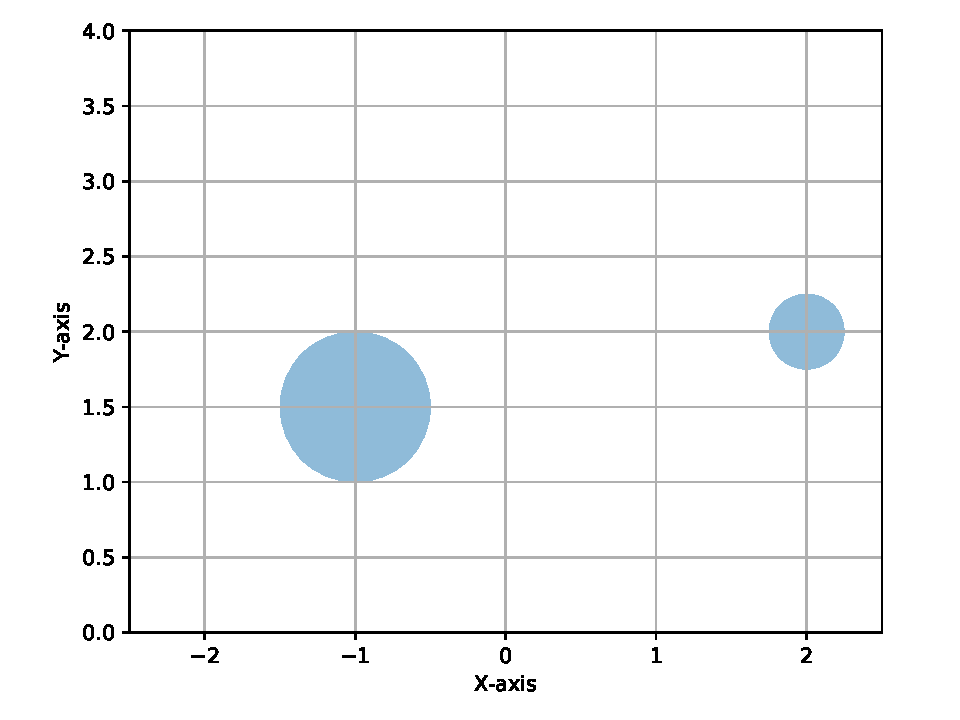
\includegraphics[width=0.5\linewidth]{../Problem 1/prob1_designated_area.pdf}
	\caption{}
	\label{fig:prob1_circles}
\end{figure}

Following the standard procedure for an RBF network, the network will have two layers. On the RBF layer, there will be two neurons, each corresponding to one of the designated regions.
As far as the output layer is concerned, there will be only a single neuron responsible for the classification output.

Moving on to some more critical parameters of the network. The centers of the RBF will be located at the same centers as the given circles, meaning at $(-1, 1.5)$ and $(-2, 2)$.
The spread ($\sigma$) needs to be chosen such that the area under the Gaussian function covers the shaded regions appropriately. 

In the absence of the exact radii of the circles, a common approach is to use the distance between the centers of the two circles to estimate the spread. The spread should typically be around the radius of the circles or slightly larger to ensure that the function covers the entire area of interest. 

The distance between the two centers can be calculated using the following equation:
\[
d = \sqrt{\left(x_2 - x_1\right)^2 + \left(y	_2 - y_1\right)^2 } = \sqrt{\left(-3\right)^2 + \left(-0.5\right)^2 } = 3.0414
\]

Since we don't want the spread to be too large to avoid overlap, we can take a fraction of this distance for each spread. If the circles are not overlapping in the classification task, we can choose the spread to be half of the distance, ensuring that each neuron's function covers its respective circle adequately.
Thus, the calculated spread is $1.52$.

Moving on to the weights of the network, we will set the weight from each RBF neuron to the output neuron to 1, assuming no overlap between the shaded regions and no need to differentiate the influence of each RBF neuron.
The weights are set to 1 to ensure that each RBF neuron's activation contributes positively and equally to the output.

Lastly, the bias of the output neuron should be set to -1, so that when neither of the RBF neurons is activated, the output neuron's activation is negative. When one or both RBF neurons are activated, the sum will be greater than 0, and the output neuron will produce a positive result.
	% !TeX spellcheck = en_US
\section{Problem 2}

We are asked to write a Python program that implements steepest descent algorithm for the 1-$S^1$-1 RBF network.
The input function that we want to approximate is 
\[
g(p) = 1 + \sin\left(p\pi/8\right), \quad \text{for} \ p \in \left[-4,4\right]
\]

We select 30 data randomly from that interval and all parameters are initialized as small numbers using \verb|numpy.random.randn| function. It returns a number at the exact specification as needed.

\begin{figure}[htbp]
	\centering
	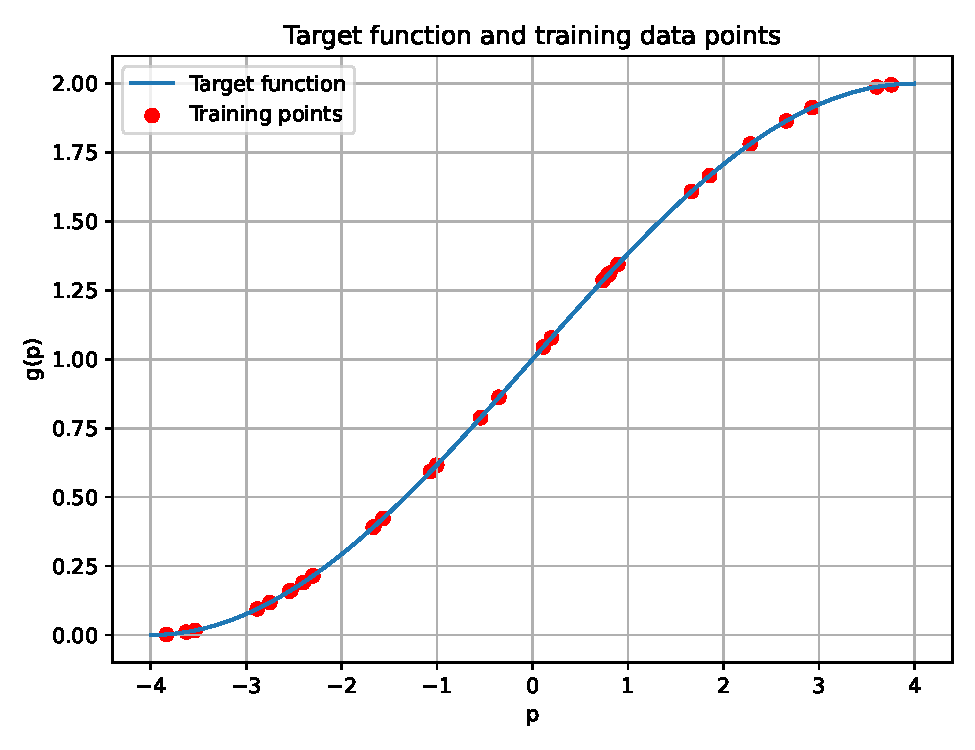
\includegraphics[width=0.6\linewidth]{../Problem 2/prob2_targetFunc_dataPoints.pdf}
	\caption{Input function in the specified area and the randomly assigned train data points.}
\end{figure}

For the randomly assigned data points, we added a custom seed number using in order for the results to be comparable but still use randomness.

	% !TeX spellcheck = en_US
\section{Problem 3}

LVQ (Learning Vector Quantization) is a type of artificial neural network algorithm used for supervised learning. It belongs to the category of competitive learning algorithms and is particularly effective for classification tasks.

\begin{figure}[htpb]
	\centering
	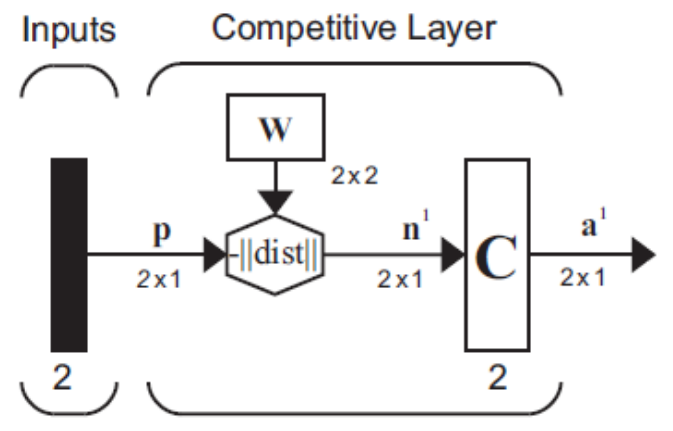
\includegraphics[width=0.4\linewidth]{../Problem 3/prob3_lvq_nn.png}
	\caption{Given neural network.}
\end{figure}

The following $-||w_i - p||$ applies to every $n^1_i$. Also, we can also state that $a^1 = compet\left(n^1\right)$, where $compet$ is competitive learning layer.

During training, the distance between $a$ and $w$ is calculated using $dist = norm\left(p-w_{1,2}\right)$ and judging by whose norm is grater, the winning neutron gets updated.
	% !TeX spellcheck = en_US
\section{Problem 4}

Problem 4 depends on Problem 3's neural network, but it is executed using different initial values.

\begin{figure}[htpb]
	\centering
	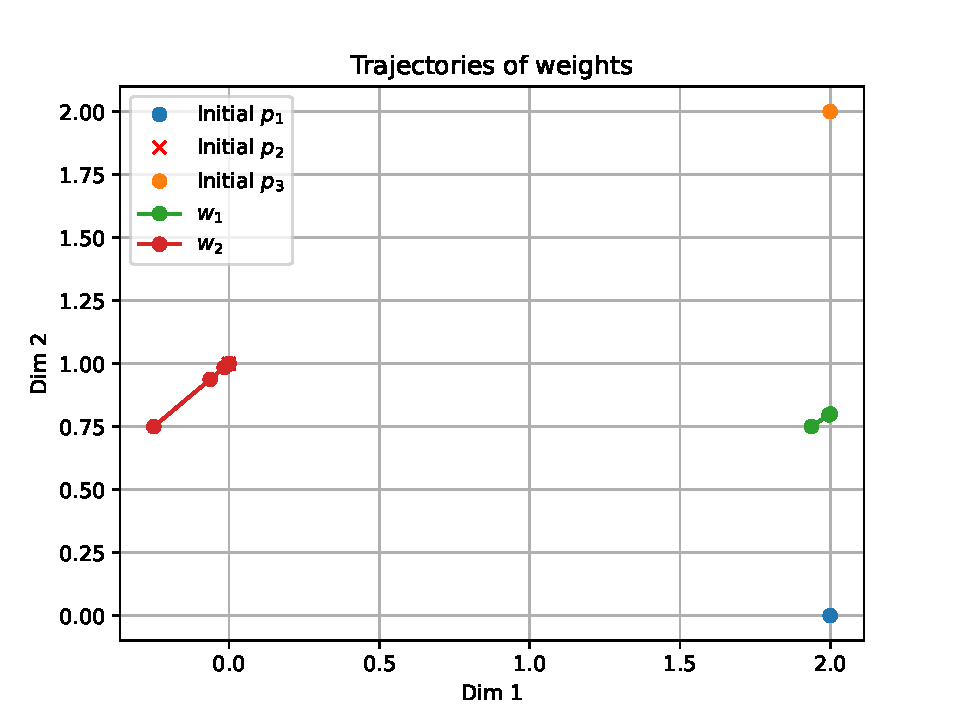
\includegraphics[width=0.5\linewidth]{../Problem 4/prob4_weights_over_epoch.pdf}
	\caption{Trajectory of weights during training.}
	\label{fig:prob4_weight_trajectory}
\end{figure}

In figure~\ref{fig:prob4_weight_trajectory}, the weight trajectory can be seen.
Based on the final weight positions after training, we can infer the clustering of the three vectors as follows:

Weight $W_1$ has moved towards and is located at the coordinates ($2.0, 0.8$), which is close to both $p_1$ ($2, 0$) and $p_3$ ($2, 2$). Given that these points are close in the input space and $W_1$ is approximately at the mean of the vertical component of $p_1$ and $p_3$, it suggests that $W_1$ would be the winning neuron for inputs similar to $p_1$ and $p_3$ in a larger number of iterations. This means that both $p_1$ and $p_3$ would be clustered together.

Weight $W_2$ has moved to a position very close to $p2$ ($0, 1$), which is at the coordinates (\num{-9.53674316e-07}, \num{9.99999046e-01}) $\approx$ ($0,1$). This indicates that $W_2$ has adjusted to represent input $p_2$.

Therefore, if the network continues to be trained for a larger number of iterations, the three vectors are likely to be clustered into two groups:

\begin{itemize}
	\item Cluster 1: Inputs $p_1$ and $p_3$, represented by $W_1$.
	\item Cluster 2: Input $p_2$, represented by $W_2$.
\end{itemize}

	% !TeX spellcheck = en_US
\section{Problem 5}

We are asked to generate an Auto Regressive (\textit{AR}) model and then create and RNN to predict it. 
Specifically, we chose to implement an LSTM as it has more parameters than GRU and is more adaptable to new information.

Samples must be generated from an AR model of the following form:
\[
X_t = 0.5 X_{t-1} - 0.1 X{t-2} + 0.2 X_{t-3} + U_t
\]
where $U_t$ is independent-identically distributed Uniform in the interval $\left( -0.25, 0.25 \right)$.

At first, we create the samples using \verb|generate_AR_data()| and the dataset for the neural network to train using \verb|create_dataset()|.

After creating all of the necessary data, we create a new model according to some predefined training sample sizes which are: $\left[100, 200, 500, 1000, 2000\right]$.
Calculation of valid loss and cost square error function is what follows the previous steps.

At the end, all cost functions are shown in figure~\ref{fig:prob5_mse}.

\begin{figure}[htpb]
	\centering
	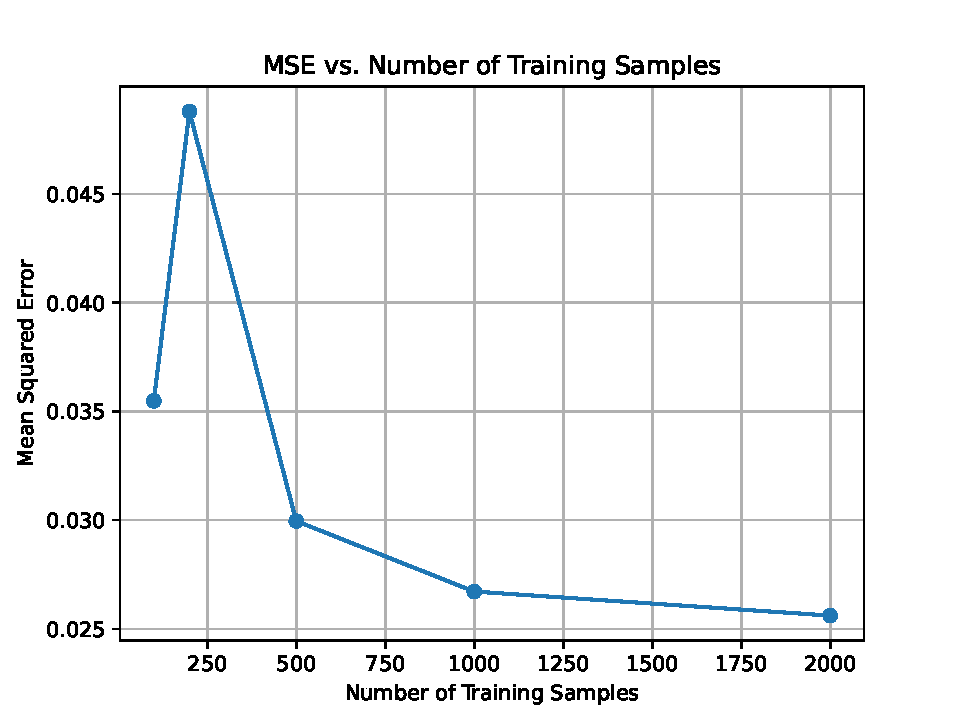
\includegraphics[width=0.5\linewidth]{../Problem 5/prob5_mse_vs_total_epoch.pdf}
	\caption{Averaged cost square error function over number of training samples}
	\label{fig:prob5_mse}
\end{figure}

The observed decrease in MSE with an increase in the number of training samples is indicative of the LSTM's capacity to learn and model the dependencies in the time series data. LSTMs are designed to capture long-term relationships, which is particularly advantageous for AR models where the future value is a function of past values.

The continuous improvement in prediction accuracy with more data suggests that the LSTM has not reached its capacity. Typically, there is a concern that a model may overfit to the training data if given too many examples.
However, in this case, overfitting does not appear to be an issue. This could be due to the stochastic nature of the AR process and the noise term, which require the model to generalize well to perform accurately.

It's also worth noting the learning dynamics of LSTM networks. During the initial phase of training, the network rapidly learns the gross features of the time series. As training progresses, the rate of improvement in MSE slows down, suggesting that the model begins to refine its understanding of finer details within the data. This refinement process requires more nuanced examples, which can only be provided by larger datasets.
	% !TeX spellcheck = en_US
\section{Problem 6}

This problem depends on Problem 5, as it uses its technique to train a neural network.
The only thing changing here is the \verb|generate_AR_data()| function, that now creates a time series that is described using the following equation:
\[
X_t = U_t + a_1 U_{t-1} + a_2 U_{t-2} + a_3 U_{t-3} + a_4 U_{t-4} + a_5 U_{t-5} + a_6 U_{t-6}
\]
with $a_1 = a_2 = 5$ and $a_3 = a_4 = a_5 = a_6 = -0.5$.

\begin{minipage}{0.48\linewidth}
	\centering
	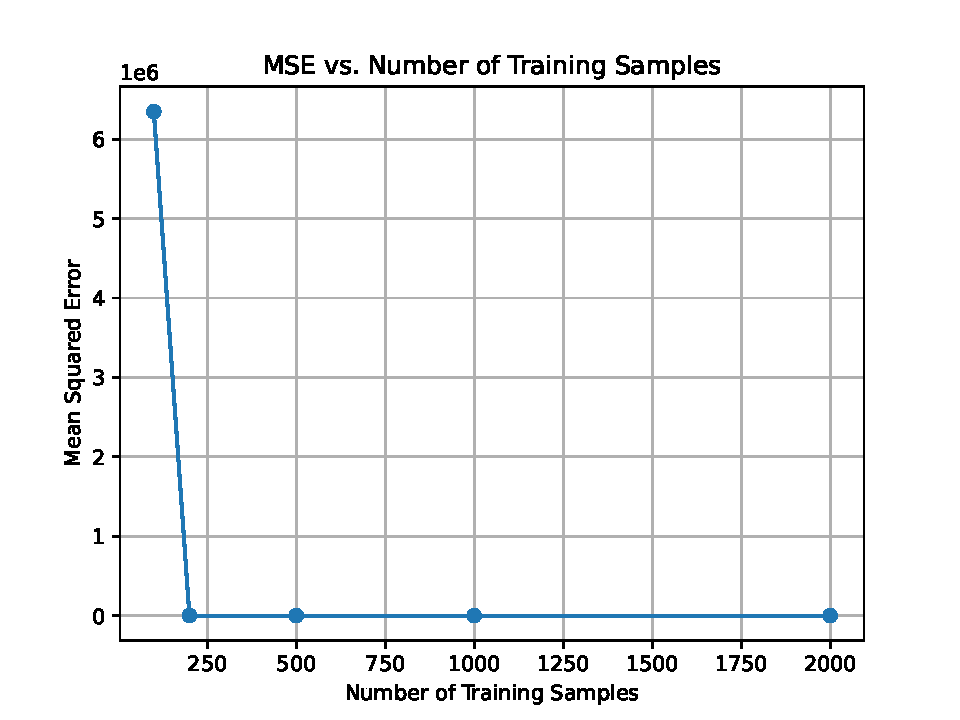
\includegraphics[width=\linewidth]{../Problem 6/prob6_mse_vs_total_epoch.pdf}
	\captionof{figure}{Averaged cost square error function over number of training samples}
	\label{fig:prob6_mse_total_epoch}
\end{minipage} \hfill
\begin{minipage}{0.48\linewidth}
	\centering
	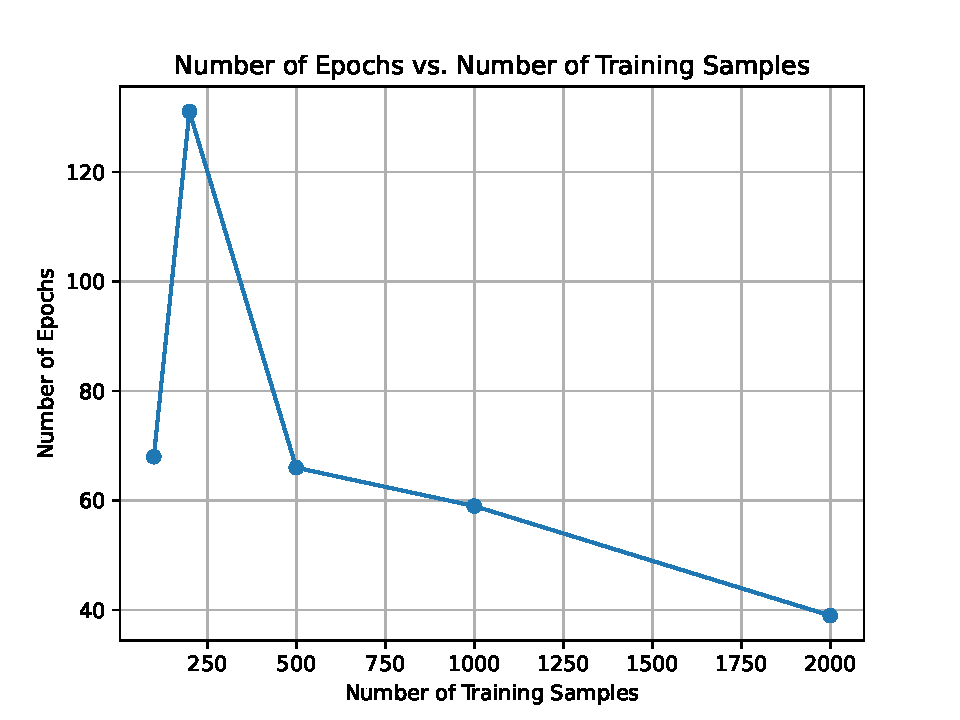
\includegraphics[width=\linewidth]{../Problem 6/prob6_epoch_vs_training_samples.pdf}
	\captionof{figure}{Number of epochs required for the NN to converge}
	\label{fig:prob6_epoch_train_samples}
\end{minipage}

	\section{Problem 7}
Modeling expressions as fuzzy subsets in the context of fuzzy logic allows us to handle the uncertainty and imprecision inherent in certain descriptions like "large," "very small," or "medium-weight." In fuzzy logic, each element of the subset has a degree of membership ranging from 0 to 1, where 0 means "not a member at all" and 1 means "fully a member".\\
Below are examples of how you might model the given expressions as fuzzy subsets using MATLAB code snippets, assuming some reasonable definitions for each term.\\

\underline{LARGE INTEGERS}\\
For "Large integers," we need a membership function that gradually increases as the integers become larger. A simple way to model this is to use a function that increases the membership score as the number exceeds a certain threshold. However, defining "large" is subjective and can vary depending on the context. For simplicity, let's assume integers greater than 100 are considered large, but the transition starts at 50, becoming more "large" as the number increases.

\begin{figure}[h]
	\centering
	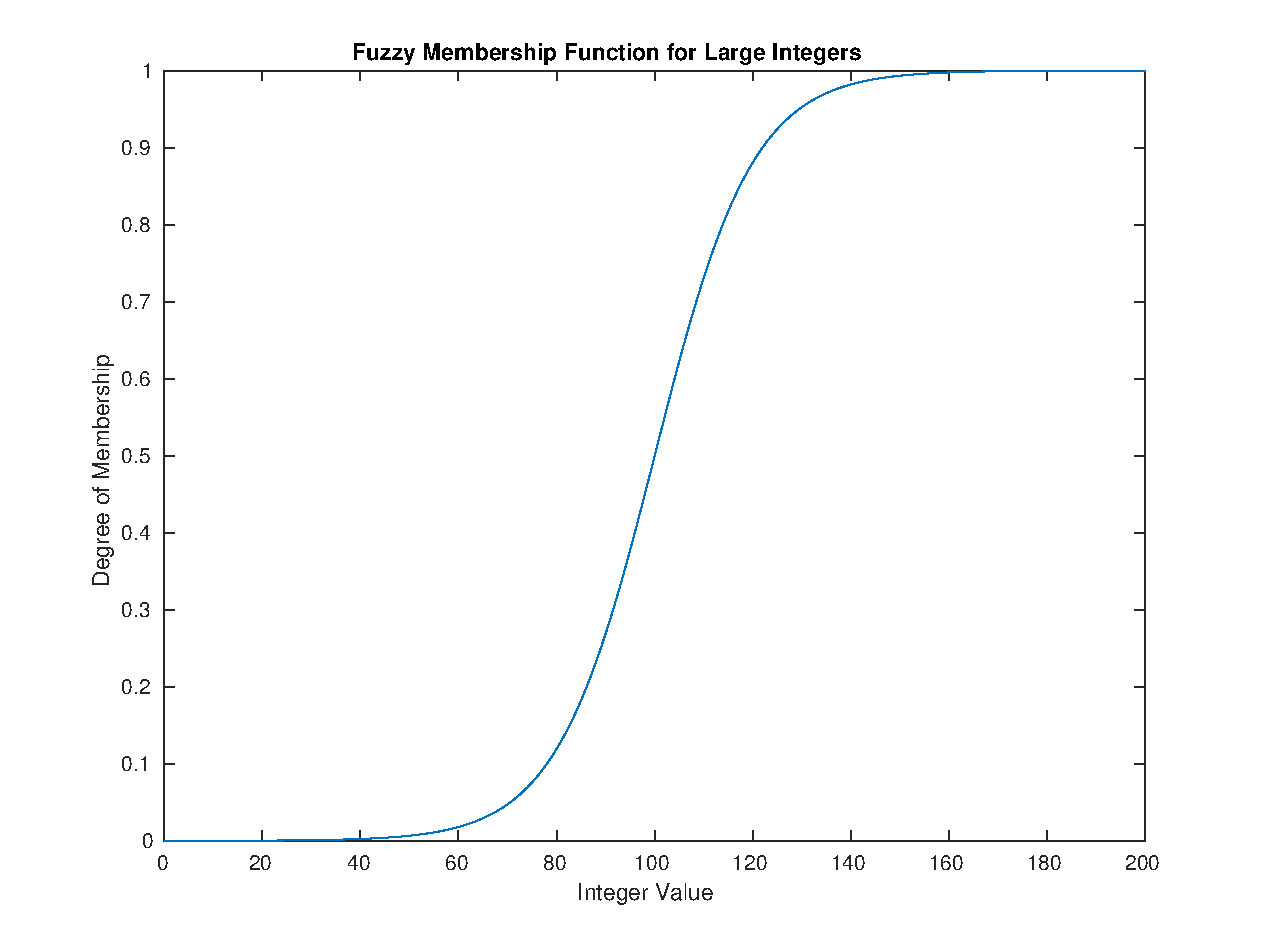
\includegraphics[width=0.6\textwidth]{../Problem 7/large_int.pdf}
	\caption{Fuzzy membership function for Large Integers}	
\end{figure}
we are using the sigmoid function for a smooth transition.
\vspace{5mm}

\underline{VERY SMALL NUMBERS}\\
For "very small numbers," we can consider numbers close to zero as having a higher degree of membership. "Very small numbers" can include both positive numbers close to zero and negative numbers. For this, a membership function that assigns higher scores to numbers closer to zero can be used. We'll focus on positive numbers for simplicity, but this can be adjusted to include negatives.

\begin{figure}[H]
	\centering
	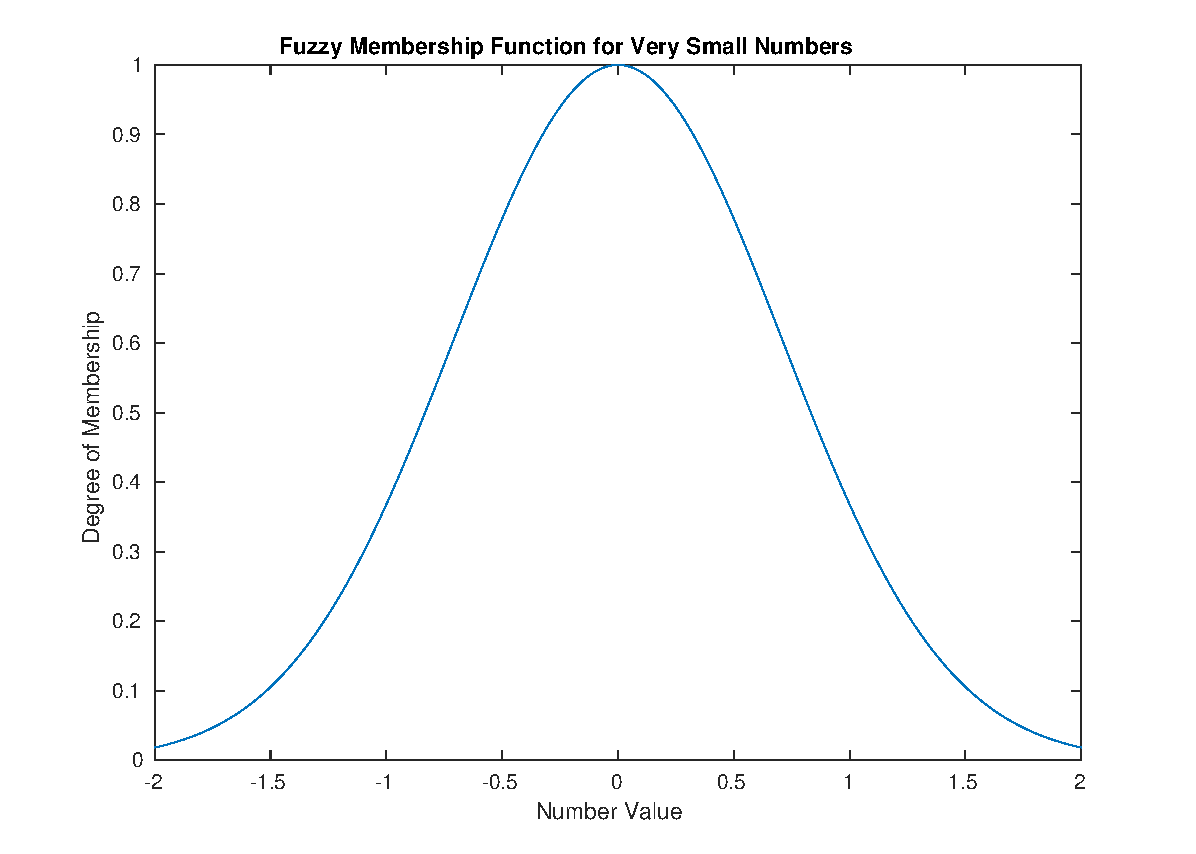
\includegraphics[width=0.6\textwidth]{../Problem 7/small_int.pdf}
	\caption{Fuzzy membership function for Very Small Numbers}	
\end{figure}
we are using the Gaussian function centered at 0.
\vspace{5mm}

\underline{MEDIUM-WEIGHT MEN}\\
Assuming the average weight range for medium-weight men is between 70kg and 90kg, with the peak at 80kg, we can define a triangular membership function.

	% !TeX spellcheck = en_US
\section{Problem 8}
The term "ordinary subset of level $\alpha$ in fuzzy set theory refers to a non-fuzzy subset that is created from a fuzzy subset by taking into consideration only those elements whose degrees of membership are at least $\alpha$. In essence, it's a threshold-based selection from a fuzzy set in which each element is only included if its membership score is greater than or equal to $\alpha$.\\
Conversely, this idea is extended to pairs of components for a fuzzy relation by the "ordinary relation of level $\alpha$". A set of ordered pairs with corresponding degrees of membership that indicate the strength of the relationship between the elements form a fuzzy relation. Thus, the set of all pairs whose membership in the fuzzy relation is at least $\alpha$ is the ordinary relation of level $\alpha$. \\

Analytically, the ordinary relation of level $\alpha$ for a fuzzy relation is defined as the set of all pairs $(x,y)$ for which the membership function $\mu_{\tilde{R}}(x,y)$ is greater than or equal to $\alpha$. Alternatively, it is a crisp set that is derived from the fuzzy relation by incorporating all element pairs with a degree of membership greater than the specified level $\alpha$\\

For a fuzzy relation with a membership function $\mu_{\tilde{R}}(x,y) = 1 - \frac{1}{1+x^2+y^2}$, the ordinary relation of level $0.3$ is the set:\\
\begin{equation}
	R_{0.3} = {(x,y) | \mu_{\tilde{R}}(x,y) \geq 0.3}
\end{equation}
This means you are looking for all the pairs $(x,y)$ where the membership value is at least $0.3$.\\

To determine analytically the ordinary relation of level $0.3$, we will solve the inequality
\begin{align*}
	\mu_{\tilde{R}}(x,y) \geq 0.3 \\
	1 - \frac{1}{1+x^2+y^2} \geq 0.3 \\
	\frac{1}{1+x^2+y^2} \leq 0.7 \\
	1 + x^2 + y^2 \geq \frac{1}{0.7} \\
	x^2 + y^2 \geq \frac{1}{0.7} - 1 \\
	x^2+y^2 \geq \frac{3}{7}
\end{align*}
From basic math we know that $	x^2 + y^2$ is the equation of a circle. This represents the region outside a circle centered at the origin with a radius of $\sqrt{\frac{3}{7}}$.This means the ordinary relation of level 
$0.3$ includes all $(x,y)$ pairs whose distance from the origin is at least 
$\sqrt{\frac{3}{7}}$.\\
To visualize this, we will plot a circle centered at the origin with a radius of 
$\sqrt{\frac{3}{7}}$.​
The area outside this circle represents the ordinary relation of level 
$0.3$.
\begin{figure}[H]
	\centering
	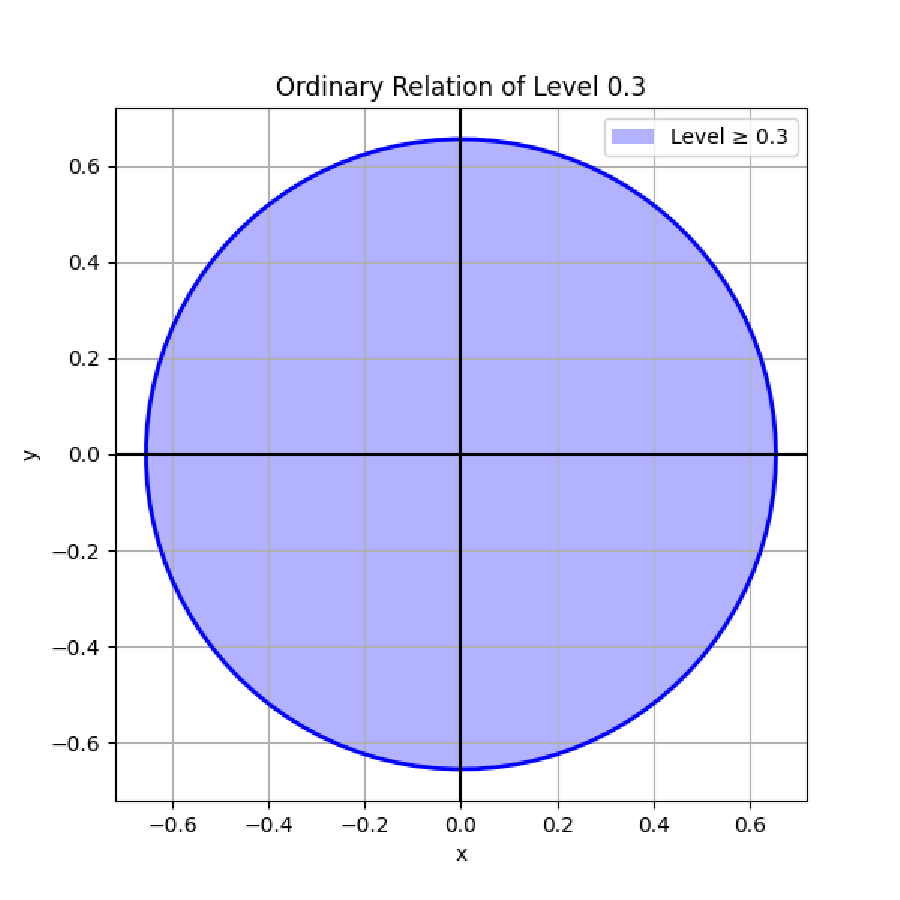
\includegraphics[width=0.5\textwidth]{../Problem 8/ordinary_plot.pdf}
	\caption{Ordinary relation of Level $0.3$}
\end{figure}
The plot above represents the ordinary relation of level $0.3$ for the given fuzzy relation. The blue shaded area, including the boundary, otside the circle indicates the region where the membership function is greater than or equal to 0.3. This area corresponds to all points $(x,y)$ whose distance from the origin is at least $\sqrt{\frac{3}{7}}$, as derived analytically. The boundary circle itself represents the exact threshold where the membership value $0.3$ and the area outside this circle encompasses all points with a membership value greater than $0.3$., fulfilling the condition for the ordinary relation of level 0.3. 
\\
The area enclosed by the circle is: Area = $1.346396851533$

	\section{Problem 9}
To calculate the index of fuzziness $v$ of a fuzzy subset $A$ defined on a fuzzy subset $A$ defined on a reference set $E = [0, \alpha] \subseteq \mathbb{R}$ with a membership function, we can use the following general formula for the index of fuzziness:
\begin{equation}
	\nu_L(\tilde{A}) = \frac{1}{|E|} \sum_{x \in E} \min(\mu_{\tilde{A}}(x), 1 - \mu_{\tilde{A}}(x))
\end{equation}
In a continuous domain, this becomes:
\begin{equation}
	\nu_L(\tilde{A}) = \frac{1}{\text{measure}(E)} \int_{E} \min(\mu_{\tilde{A}}(x), 1 - \mu_{\tilde{A}}(x)) \, dx
\end{equation}

\underline{Question A}\\
Given the specific membership function $\mu_{\tilde{A}}(x) = \dfrac{x^2}{\alpha^2}$, for $x \in [0, \alpha]$ and assuming $E = [0, \alpha]$ the linear index of fuzziness can be calculated directly because the measure of $E$ is $α$. Therefore, the formula for the linear index of fuzziness over the interval 
$[0,α]$ is:
\begin{equation}
	\nu_L(\tilde{A}) = \dfrac{1}{\alpha} \int_{0}^{\alpha} \min\left( \dfrac{x^2}{\alpha^2}, 1 - \dfrac{x^2}{\alpha^2} \right) dx
\end{equation}
However, since $\dfrac{x^2}{\alpha^2}$ increases monotically from $0$ to $1$ as $x$ goes from $0$ to $\alpha$. and the function $\min\left(\frac{x^2}{\alpha^2}, 1 - \frac{x^2}{\alpha^2}\right)
$ is symmetric around $x = \dfrac{\alpha}{\sqrt{2}}$, where $\dfrac{x^2}{\alpha^2} = 1 - \dfrac{x^2}{\alpha^2}$, the integral simplifies to $2$ times the integral from $0$ to $\dfrac{\alpha}{\sqrt{2}}:$
\\
\begin{gather}
	\nu_L(\tilde{A}) = \frac{2}{\alpha} \int_{0}^{\frac{\alpha}{\sqrt{2}}} \frac{x^2}{\alpha^2} \, dx \\
	\nu_L(\tilde{A}) = \frac{2}{\alpha^3} \int_{0}^{\frac{\alpha}{\sqrt{2}}} x^2 \, dx\\
	\nu_L(\tilde{A}) = \frac{2}{\alpha^3} \left[ \frac{x^3}{3} \right]_{0}^{\frac{\alpha}{\sqrt{2}}} \\
	\nu_L(\tilde{A}) = \frac{2}{\alpha^3} \cdot \frac{\left(\frac{\alpha}{\sqrt{2}}\right)^3}{3}\\
	\nu_L(\tilde{A}) = \frac{2}{\alpha^3} \cdot \frac{\alpha^3}{3\sqrt{8}} \\
	\nu_L(\tilde{A}) = \frac{\sqrt{2}}{3}
\end{gather}
This result represents the linear index of fuzziness of $A$ which is independent of $\alpha$ due to the normalization over the interval $[0,\alpha]$.



	\section{Problem 10}
The min-max composition of fuzzy relations is a method for combining two fuzzy relations to produce a new fuzzy relation. The process is somewhat analogous to matrix multiplication in linear algebra but uses the "min" and "max" operations instead of multiplication and addition. \\
Given two fuzzy relations $R1$ and $R2$, with membership functions $\mu_{\tilde{R1}}(x,y)$ and $\mu_{\tilde{R2}}(y,z)$ respectively, the min-max composition $R = R1 \circ R2 $ has a membership function defined for each pair $(x,z)$ by:
\begin{equation}
	\mu_R(x, z) = \max_{y} \min(\mu_{R1}(x, y), \mu_{R2}(y, z)
\end{equation}

In order to gain a deeper understanding, , we will analyse the expression
\begin{itemize}
	\item $\min(\mu_{R1}(x, y), \mu_{R2}(y, z)$: For a fixed $x$ and $z$, and for each intermediate value of $y$, we must calculate the minimum membership value between 
	$\mu_{\tilde{R1}}(x,y)$ and $\mu_{\tilde{R2}}(y,z)$ . This minimum value represents the strongest constraint on the relationship between $x$ and $z$ via the intermediary $y$.
	\item $\max_{y} $: Select the maximum value out of all these minimum values as the membership degree for the pair $(x,z)$ in the relation $R$.
\end{itemize}

Now, let's analyze the exponential terms within the membership functions. We have:
\begin{align}
	\mu_{\tilde{R1}}(x,y) = e^{-k(x - y)^2}, \quad \text{for } k \geq 1 \\
	\mu_{\tilde{R2}}(y,z) = e^{-k(y - z)^2}, \quad \text{for } k \geq 1
\end{align}
The exponential function $e^{-k(w)^2}$  is a Gaussian function that has its maximum value when 
$w=0$ and decreases as $w$ moves away from $0$ in either direction. This means that for a fixed 
$x$ and $z$, the membership values $\mu_{\tilde{R1}}(x,y)$ and $\mu_{\tilde{R2}}(y,z)$ will be higher when $y$ is close to $x$ and $z$ respectively, because the terms $(x-y)^2$ and $(y-z)^2$ will be smaller, making the exponent closer to $0$.\\

When we take the minimum of these two membership values, we are essentially looking for the point where the overlap between the two functions is the greatest, since the minimum value is dominated by the smaller of the two membership degrees.
\\

In other words, since the membership functions involve an exponential function of a squared term, the minima will occur where the arguments of the exponential functions are closest to each other, that is, when $(x-y)^2$ and $(y-z)^2$
are minimal.
\\

Graphically, we can represent the membership functions $\mu_{R1}$ and $\mu_{R2}$ as surfaces over $x-y$ and $y-z$ planes, respectively. The composition $\mu_R$ would be a new surface over the $x-z$ plane, which is derived from the "peaks" of the minimum values between the two original surfaces for every $x$ and $z$. We will assume a value for $k$ to proceed with the calculation. Let's set $k=1$ for simplicity. We will first define the membership functions and then compute the max-min composition for a range of 
$x$ and 
$z$ values.

\begin{figure}[H]
	\centering
	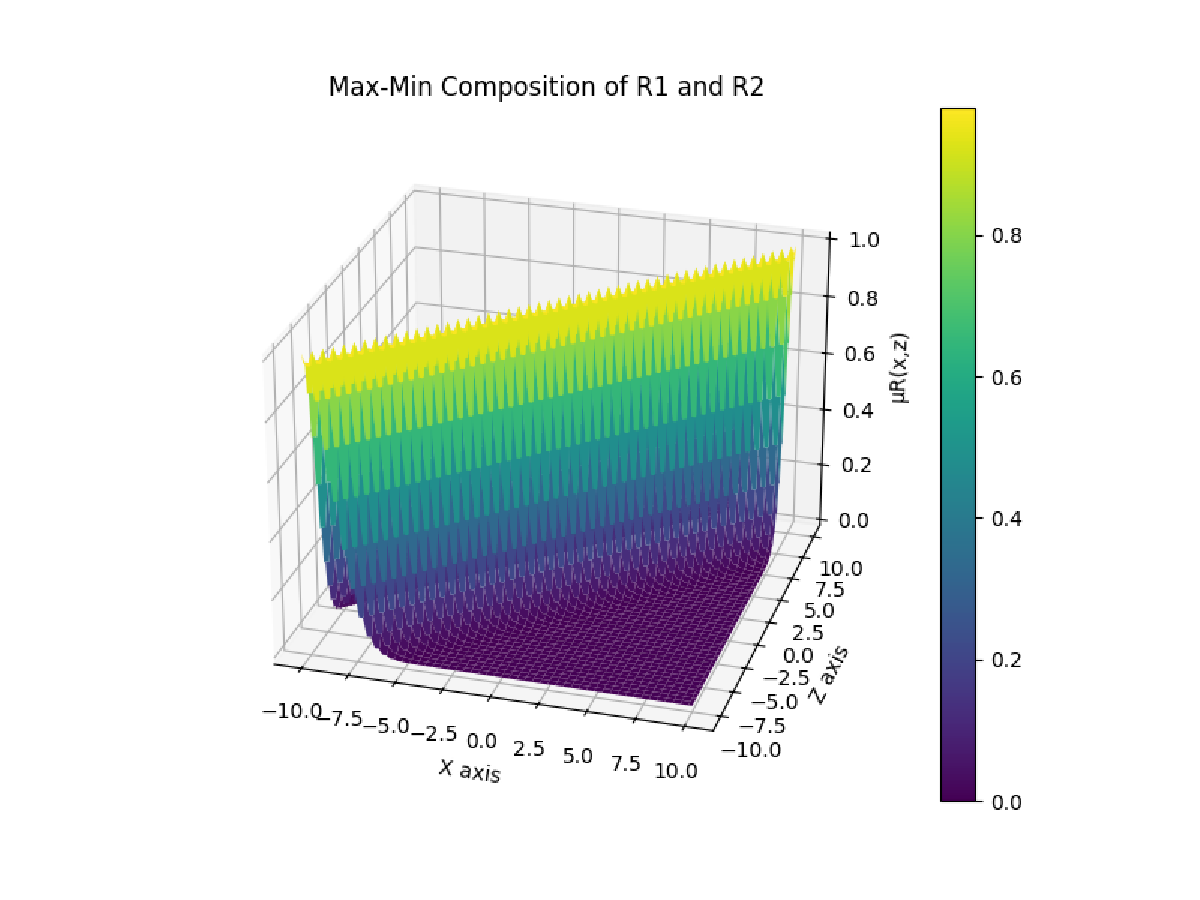
\includegraphics[width=0.8\textwidth]{../Problem 10/minmax_plot.pdf}
	\caption{Max-Min Composition of Fuzzy Relations R1 and R2}
\end{figure}
	

	
	
\end{document}